\chapter{Liga RoboCup \label{chap:robocup}}
\section{Opis projektu RoboCup \label{sec:opis_robocup}}
	Jak już wspomaniano we wstępie, głównym celem rozgrywek \emph{RoboCupSoccer} jest stworzenie do 2050 roku drużyny w pełni autonomicznych robotów humanoidalnych zdolnych wygrać rozgrywkę z aktualnymi mistrzami 
	świata.
	W niniejszej pracy problematyka rozgrywek robotów w piłkę nożną zostanie przedstawiona jedynie skrótowo. Skupiono się na omówieniu
	budowy robota wykorzystywanego w lidze, którą starano się odwzorować. Więcej informacji na temat projektu RoboCup można znaleźć w pracy inżynierskiej \cite{inzynierka} lub 
	na oficjalnej stronie projektu \mbox{\url{http://www.robocup.org}}.
	Kluczową rolę w realizacji postawionego zadania pełni konstrukcja zarówno mechaniczna jak i elektroniczna
	robota. Zawodnik powinien być wyposażony w odpowiedni zestaw czujników umożliwiających osiągnięcie pełnej autonomiczności. 
	Osobnym problemem jest opracowanie funkcjonalnego oprogramowania umożliwiającego koordynację działań wielu robotów.
	Projekt RoboCup jest realizowany nieprzerwanie od września 1993 roku, a mistrzostwa odbywają się regularnie w różnych miejscach na świecie.
	Rozgrywki toczone są w kilku niezależnych od siebie ligach. Aktualnie wyróżnione zostały następujące ligi:
	\begin{itemize}
	\item \emph{Soccer Simulation League}
	\item \emph{Small-size League}
	\item \emph{Middle-size League}
	\item \emph{Standard Platform League }
	\item \emph{Humanoid League}
	\end{itemize}
	
	\emph{Soccer Simulation League} jest pewnego rodzaju grą, w której uczestniczące drużyny implementują program decydujący o zachowaniu zawodników.
	Jest ona najstarszą z lig, która towarzyszy przedsięwzięciu od samego początku jego istnienia.
	Zachowanie robotów jest symulowane za pomocą programu zwanego \emph{RoboCup Soccer Simulator}.
	\begin{figure}[b]
	\centering
	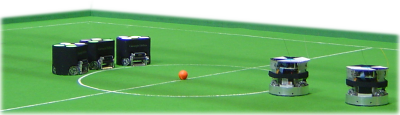
\includegraphics[scale=0.6]{./liga_robocup/F180}
	\caption{ Roboty biorące udział w \emph{Small-Size League}\newline(źródło: \texttt{www.robocup.org})} \label{fig:F180}
	\end{figure}
	
	Kolejną z lig jest \emph{Small-Size League}. W rozgrywkach tej ligi drużyna składa się maksymalnie z pięciu niewielkich robotów, takich jak widoczne na fotografii \ref{fig:F180}. 
	Roboty  nie są jednak w pełni autonomiczne, ponieważ nie posiadają własnych sensorów wizyjnych. Algorytm sterujący czerpie informację o~położeniu piłki oraz robotów z~globalnego systemu
	wizyjnego \textit{SSL-Vision} składającego się z szeregu kamer umieszczonych nad boiskiem. Każde z boisk, na którym toczone są rozgrywki jest wyposażone w ten system. Drużyna odbiera już przetworzone
	informacje o położeniu i prędkościach robotów oraz piłki.
	Lidze tej został poświęcony w całości paragraf~\ref{sec:F180}.	

	\emph{Middle-size League} to rozgrywki w pełni autonomicznych robotów. W przeciwieństwie do poprzedniej ligi, globalny system wizyjny jest całkowicie zakazany.
	Każdy robot jest wyposażony w osobny zestaw czujników wizyjnych. Zawodnicy niezależnie muszą reagować na zmieniającą się sytuację na planszy oraz
	wspólnie dążyć do wypracowania strategii determinowanej przez zachowania pozostałych graczy.

	W projekcie wyróżnione są także ligi \emph{Standard Platform League }, czyli rozgrywki piesków \textit{Aibo}, konstruowanych przez firmę \textit{Sony} oraz 
	liga robotów humanoidalnych. W tej ostatniej biorą udział roboty przypominające swoją budową ludzi, czyli posiadające korpus, nogi, ręce oraz głowę.
	\section{Szczegółowe omówienie ligi Small-size (F180) \label{sec:F180}}
	\subsection{Zasady}
	Corocznie przed nowymi mistrzostwami wydawany jest nowy regulamin, który będzie na nich obowiązywać. Zmiany nie są zazwyczaj daleko idące, modyfikacje dotyczą głównie rozmiaru boiska.
	W poprzednich latach dopuszczono możliwość stosowania przez drużyny własnego globalnego systemu udostępniającego informację o położeniu i prędkości zawodników.
	Jednak od $2010$ roku sprawę systemu wizyjnego usystematyzowano, stworzono system o nazwie \textit{SSL-Vision}, który jest obowiązkowy w lidze. 
	Całkowity rozmiar boiska, wliczając w to pola autowe, jest równy 7.4~[m] na 5.4~[m], natomiast sama plansza, na której toczona jest rozgrywka ma wymiary 6.05~[m] na 4.05~[m].
	Powierzchnia jest równa i  wyłożona zielonym dywanem lub wykładziną. Podczas meczu wykorzystywana jest standardowa piłka do golfa koloru pomarańczowego. Jej promień jest równy 43~[mm], a masa
	46~[g].
	Uczestniczące drużyny mogą składać się maksymalnie z pięciu robotów, jeden z nich może zostać oddelegowany do pełnienia
	funkcji bramkarza, jednak powinno to zostać zgłoszone przed rozpoczęciem meczu. W trakcie rozgrywki roboty mogą być wymieniane na nowe, tak samo jak w rzeczywistym meczu.  
	Sytuacja taka musi także musi być zgłoszona wcześniej arbitrowi.
	\begin{figure}[h!]
	\centering
	\includegraphics[ scale=0.5]{./liga_robocup/referee_box}
	\caption{Program wykorzystywany przez sędziego w  \mbox{\emph{Small Size League}}\newline(źródło: \texttt{www.robocup.org}) }
	\label{fig:referee_box}
	\end{figure} 
	Konstrukcja mechaniczna robota nie jest mocno ograniczona, zalecenia dotyczą głównie wymiarów. Robot powinien zmieścić się w walcu o średnicy 18~[cm] oraz wysokości 15~[cm].
	Dodatkowo może on być wyposażony w urządzenie do prowadzenia piłki - \textit{dribbler}. Tutaj jednak istnieją pewne ograniczenia dotyczące
	samej budowy urządzenia oraz wykorzystywania go w czasie gry. Zawodnik nie może pokonać z piłką odległości większej niż 50~[cm]. Po przejechaniu takiego dystansu powinien zdecydować się
	na podanie jej innemu zawodnikowi lub oddanie strzału na bramkę. Może również zdecydować się na kopnięcie jej przed siebie i dalsze podążanie w jej kierunku. Niedostosowanie się do tych zasad powoduje sygnalizowanie przez arbitra
	przewinienia oraz wykonanie rzutu wolnego przez drużynę przeciwną. Konstrukcja urządzenia do dryblowania nie powinna także uniemożliwiać kontaktu z piłką zawodnikowi drużyny przeciwnej.

	Przebieg rozgrywki robotów kontroluje arbiter. Jego zadaniem jest czuwanie nad przestrzeganiem obowiązującego regulaminu. Sygnalizuje on przewinienia, przyznaje punkty za zdobyte bramki
	oraz wykrywa inne nietypowe sytuacje, jakie mogą wydarzyć się podczas meczu. Decyzja sędziego, tak jak w rzeczywistym meczu, może zostać zmieniona po konsultacjach z asystentem.
	Arbiter komunikuje się z zawodnikami za pomocą programu, którego interfejs użytkownika zamieszczono na rysunku \ref{fig:referee_box} .

	Wszystkie akcje sędziego wprowadzone do tego programu są udostępniane specjalnym protokołem zawodnikom, dzięki temu rozgrywka nie wymaga ludzkiej ingerencji.
	\subsection{Schemat komunikacji}
	Kluczową sprawą podczas rzeczywistej rozgrywki jest dostęp do informacji o położeniu piłki
	i pozostałych robotów. Jak już wspomniano wcześniej organizacja udostępnia drużynom w tym celu system \textit{SSL-Vision}. Uproszczony schemat systemu
	wizyjnego widoczny jest na rysunku~\ref{fig:comunication}.
	Składa się on z kamery ustawionej centralnie nad boiskiem oraz ze specjalnej aplikacji \mbox{\emph{SSL-Vision}}\footnote{ Do pobrania z \url{http://code.google.com/p/ssl-vision}}.
	Obecnie w skład systemu może wchodzić kilka kamer.
	Obraz zarejestrowany przez kamery jest przesyłany do komputera, gdzie jest przetwarzany przez \emph{SSL-Vision} w czasie rzeczywistym. Program dostarcza informację 
	o położeniu oraz o prędkościach robotów i piłki. Dane te następnie są wykorzystywane przez rywalizujące ze sobą drużyny na potrzeby ich algorytmów.
	Algorytm sterujący drużyną jako wynik swojego działania powinien zwracać kierunek i prędkość zawodników. Informacje te wysyłane są droga radiową do robota.
	\begin{figure}[H]
	\centering
	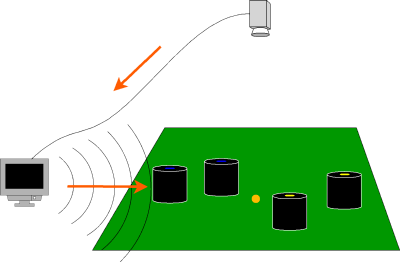
\includegraphics[ scale=0.5]{./liga_robocup/dataflow}
	\caption{Schemat komunikacji w  \mbox{\emph{Small Size League}}\newline(źródło: \texttt{www.robocup.org}) }
	\label{fig:comunication}
	\end{figure} 	
	System \mbox{\emph{SSL-Vision}} poza określaniem położenia poszczególnych zawodników na boisku, może także określać ich orientację na
	płaszczyźnie. W tym celu roboty wyposażone są w specjalne, wielokolorowe znaczniki. Przed rozpoczęciem meczu, zawodnicy każdej z drużyn oznaczani są za pomocą wylosowanej pary kolorów, 
	które zawiera znacznik. Zastosowanie dwukolorowych znaczników umożliwia określanie orientacji robotów.bab.

\section{Budowa robota \label{sec:budowa_robota} w \emph{Small-size League}}
	W oficjalnych zasadach ligi \emph{Small-size League} model zawodnika nie jest dokładnie sprecyzowany, uczestniczące drużyny mogą zatem korzystać z przygotowanych przez siebie robotów.
	Regulamin określa jedynie maksymalne wymiary robota mogącego brać udział w rozgrywce oraz sposób prowadzenia piłki. Analizując jednak budowę zawodników uczestniczących w mistrzostwach
	w ostatnich latach, szybko można zauważyć, że wśród zgłaszanych drużyn dominuje jedna konstrukcja mechaniczna.
	Została ona zaprezentowana na  rysunkach \ref{fig:F180_budowa}.
	\begin{figure}
	\centering
	\subfloat[]{\label{fig:F180_budowa1}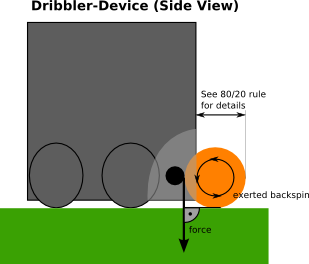
\includegraphics[ scale=0.34]{./liga_robocup/F180_budowa1}}
	\subfloat[]{\label{fig:F180_budowa2}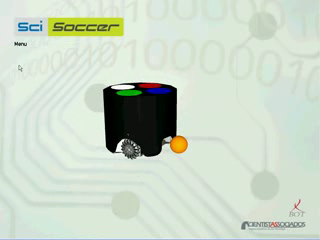
\includegraphics[ scale=0.38]{./liga_robocup/F180_budowa2}}
	\subfloat[]{\label{fig:F180_budowa3}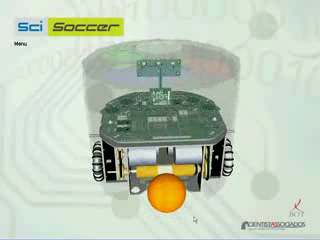
\includegraphics[ scale=0.38]{./liga_robocup/F180_budowa3}}
	\caption{Popularny model robota wykorzystywany w \mbox{lidze \emph{F180}}\newline(źródło: \texttt{www.robocup.org}) }
	\label{fig:F180_budowa}
	\end{figure}
	Zaprezentowane rozwiązanie wykorzystuje omnikerunkową bazę jezdną. Podejście takie jest bardzo praktyczne, gdyż umożliwia ono zmianę orientacji zawodnika w miejscu, co jest często
	spotykanym manewrem podczas gry w piłkę nożną. Robot porusza się na trzech niezależnie napędzanych kołach szwedzkich. Zastosowanie kół tego typu jest kluczowe dla osiągnięcia wielokierunkowości
	bazy jezdnej. Koło szwedzkie, poza obrotem wokół własnej osi umożliwia także obrót wokół punktu styczności koła z podłożem oraz wokół osi rolek umieszczonych na kole.
	
	Zawodnik rozgrywek powinien być także wyposażony w urządzenie umożliwiające prowadzenie piłki. Stosowana przez drużyny konstrukcja mechaniczna zawiera urządzenie do dryblowania. Jest ono zaprezentowane
	na rysunkach \ref{fig:F180_budowa1} oraz \ref{fig:F180_budowa3}. 
	\textit{Dribbler} zbudowany jest z walca, który obracając się nadaje piłce wsteczną rotację, dzięki temu nie odbija się ona od robota w momencie podania.
	Urządzenie umożliwia robotowi kontrolowanie piłki podczas hamowania lub obracania się.
	\begin{wrapfigure}{r}{0.42\textwidth}
	\vspace{-20pt}
	\begin{center}	
	\includegraphics[width=0.3\textwidth]{./liga_robocup/robocup_markers}
	\end{center}
	\caption{Znacznik umożliwiający systemowi wizyjnemu identyfikację robotów \newline(źródło: \texttt{www.robocup.org})\label{fig:znacznik}}
	\vspace{-10pt}
	\end{wrapfigure}
	W regulaminie rozgrywek dopuszczono do stosowania jedynie urządzenia do dryblowania działające na piłkę siłą prostopadłą do podłoża rys.~\ref{fig:F180_budowa1} (we wcześniejszych latach
	w użyciu były urządzenia, w których obracany walec był umieszczony pionowo).

	Jak już wspomniano we wcześniejszym paragrafie, każdy uczestniczący w rozgrywce robot musi być wyposażony w znacznik (por. rys.~\ref{fig:znacznik}).
	Umieszczony jest on w takim miejscu, aby kamery współpracujące z systemem \mbox{\emph{SSL-Vision}} mogły go zarejestrować (przykrywa robota od góry).
	Dzięki znacznikom system wizyjny może określać przynależność robotów do poszczególnych drużyn, a także rozpoznawać ich pozycję, orientację na płaszczyźnie oraz prędkość.